\chapter*{Instalasi Anaconda}

\begin{enumerate}
	\item Ketika selesai mendownload akan keluar seperti digambar. Lalu klik run untuk melanjutkan 			penginstalan 
	\begin{figure} [h]
	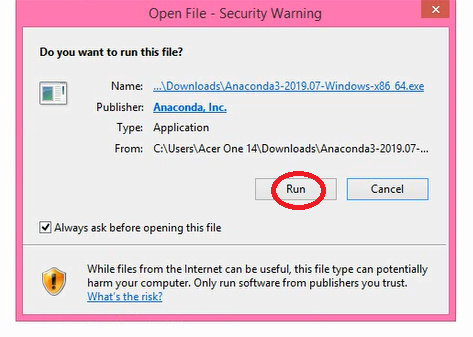
\includegraphics[width=5cm]{python/1.png}
	\centering
	\end{figure}
	
	\item lalu menunggu setup loading seperti digambar 
	\begin{figure} [h]
	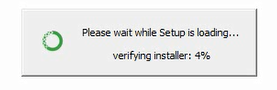
\includegraphics[width=5cm]{python/2.png}
	\centering
	\end{figure}

	\item lalu klik next untuk melanjutkan 
	\begin{figure} [h]
	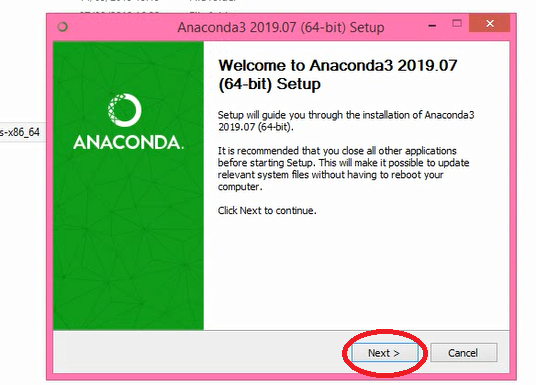
\includegraphics[width=5cm]{python/3.png}
	\centering
	\end{figure}
	
	\item Klik I agree seperti yang dibulatkan
	\begin{figure} [h]
	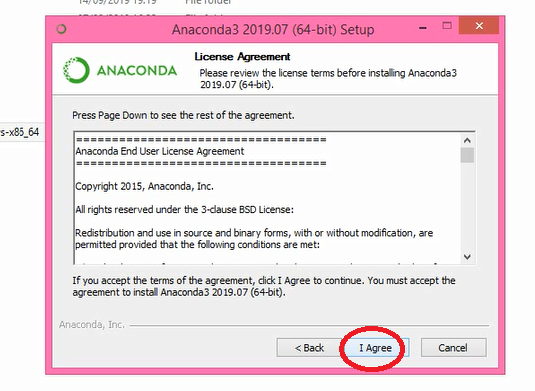
\includegraphics[width=5cm]{python/4.png}
	\centering
	\end{figure}
	
	\item Klik "Just me" agar yang dapat menggunakan kita sendiri
	\begin{figure} [h]
	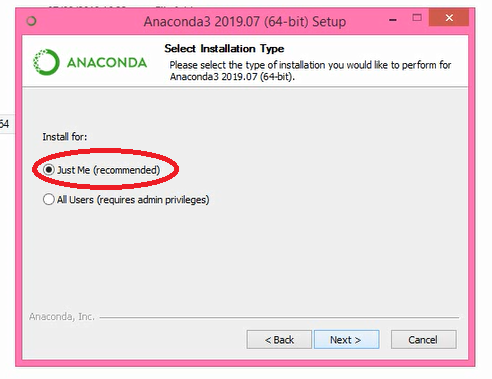
\includegraphics[width=6cm]{python/5.png}
	\centering
	\end{figure}
	
	\item Klik Next pada yang dilingkari merah, berfungsi untuk menentukan dimana file nya akan tersimpan 
	\begin{figure} [h]
	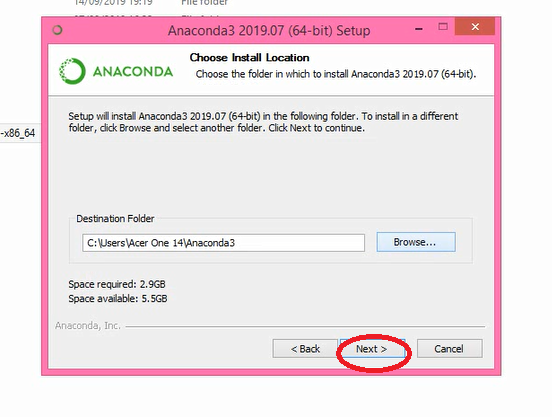
\includegraphics[width=6cm]{python/6.png}
	\centering
	\end{figure}
	
	\item Klik ceklis di kedua opsi dan lanjutkan dengan mengklik Next  
	\begin{figure} [h]
	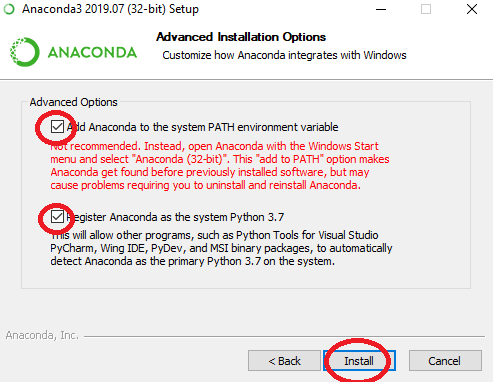
\includegraphics[width=6cm]{python/7.png}
	\centering
	\end{figure}
	
	\item lalu klik next pada 
	\begin{figure} [h]
	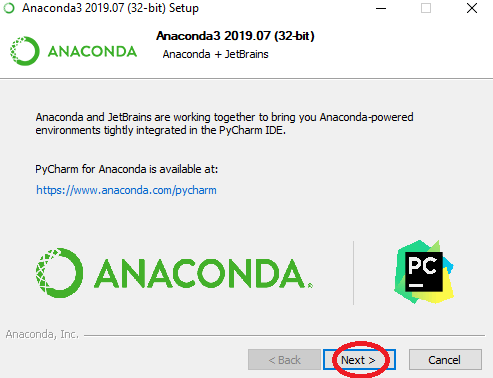
\includegraphics[width=6cm]{python/9.png}
	\centering
	\end{figure}
	
	\item dan peng-instalan selesai klik "finish" yang terdapat pada gambar 
	\begin{figure} [h]
	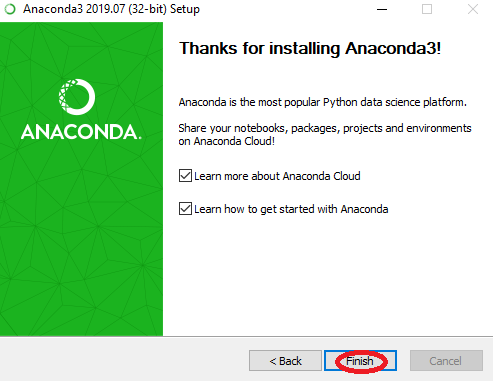
\includegraphics[width=6cm]{python/10.png}
	\centering
	\end{figure}

\end{enumerate}
